%!TEX root = reference.tex
\chapter{Packages and Libraries}
\label{packages}
\index{package@\q{package} structure}
A \ntRef{Package} represents a `unit of compilation' -- i.e., the contents of a source file. 

\index{libraries}
\Sr libraries are built using a combination of \ntRef{Package}s and catalogs. A catalog is a mapping from names to locations that is used to inform the \Sr language system of the physical locations of \ntRef{Package}s.

\section{Package Structure}
\label{packageStructure}
\index{what is in a package@what is in a \q{package}}

A \ntRef{Package} consists of the identification of the package and a set of \ntRef{Definition}s enclosed in braces. For example, the text:
\begin{lstlisting}
hello is package{
  hello() is "hello";
}
\end{lstlisting}
defines a \q{package} -- called \q{hello} -- that contains a single function -- also called \q{hello}.

\begin{aside}
The name of a \ntRef{Package} must be reflected in the name of the physical file that contains the source text. In particular, if a file contains the package \q{\emph{P}}, then the name of the file should take the form:
\begin{lstlisting}[language=bash]
.../Directory/P.star
\end{lstlisting}
\end{aside}

The body of the \ntRef{Package} may contain \ntRef{Definition}s which may also include \ntRef{ImportStatement}s.

\begin{figure}[htbp]
\begin{eqnarray*}
\ntDef{Package}&\arrow&\ntRef{Identifier}\ \q{is}\ \q{package\{}\,\ntRef{Definition}\sequence{;}\ntRef{Definition}\ \q{\}}
\end{eqnarray*}
\caption{Package Structure}\label{packageFig}
\end{figure}

A \ntRef{Package} consists of all the elements that are defined in a package source:
\begin{itemize}
\item The types defined with the source unit
\item The functions and other variables defined
\item Macros and other meta-rules (such as validation rules)
\item Operator definitions
\end{itemize}


\subsection{Top-level Variables}
\label{packageVariable}
\index{top-level variable}

Any variable that is defined at the top-level of a \ntRef{Package} is assumed to be \emph{global} across all uses of the package.

This has implications especially for top-level reassignable variables. If such a variable is changed then all importing packages will `see' the changed value.
\begin{aside}
Such shared global variables should be used sparingly if the programmer is to avoid unnecessary bugs.
\end{aside}


\subsection{Managing Exposed Elements of a Package}
By default, all the elements that are defined in a \q{package} are exported as part of the \q{package}. However, like other \ntRef{ThetaEnvironment}s, elements of the package that are marked \q{private} are not exported: i.e., they will not be visible when the package is imported.


\section{Importing}
\label{packageImport}
A \q{package} may use another package by \q{import}ing it. The \q{import} statement  denotes a requirement that the types, programs and other elements of the \q{import}ed package are made available to the importing package.

In addition to the \q{import} statement, the \q{java} statement allows access to programs defined in Java -- see Section~\vref{javaImport}.

\subsection{The \q{import} statement}
\label{import}
The \q{import} statement is used to denote that the exported elements of a package should be made available within a package. There are two variants of the \ntRef{ImportStatement}: the `open \q{import}' and the `named \q{import}'. In addition, the package to be imported may be specified by name or by URI.

\begin{figure}[htbp]
\begin{eqnarray*}
\ntDef{ImportStatement}&\arrow&[\,\q{private}\,]\ \q{import}\ \ntRef{PackageRef}\\
&\choice&\ntRef{Identifier}\ \q{is}\ \q{import}\ \ntRef{PackageRef}\\
\ntDef{PackageRef}&\arrow&\ntRef{Identifier}\\
&\choice&\ntRef{String}
\end{eqnarray*}
\caption{Import Package Statement}
\label{importStatementFig}
\end{figure}

\begin{aside}
The \ntRef{String} variant of the \q{import} must take the form of a URI string. For example, to import the package located in the file \q{pkg.star} in the same directory as the referencing package, use the form:
\begin{lstlisting}
import "pkg.star"
\end{lstlisting}
\end{aside}

\begin{aside}
Not all installations of the language system are required to support the same set of URI schemes. However, all must support the standard schemes shown in Table~\vref{standardURISchemes}. See Section~\vref{resources} for a discussion on resources and URIs.
\end{aside}

\subsubsection{Open Import}
\label{openImport}
\index{import@\q{import}!open}
An \ntRef{ImportStatement} of the form:
\begin{lstlisting}
import Pkg
\end{lstlisting}
imports all the definitions that are located with the \q{Pkg} and declares them as being at the \emph{same} scope level as other \ntRef{Definition}s within the package. 

\begin{aside}
Note that it is possible, this way, for a \q{package} to implicitly \emph{re-export} some elements of \q{package}s that the \q{package} imports.
\end{aside}

This has two primary implications: all the exported definitions may be used without qualification as though they had been defined locally. However, if a given name is declared twice -- even if in two separate packages -- then the compiler will show an error.

In addition to the regular functions and types defined in the imported package, any contracts, macros and operator definitions that are defined in the imported package are also `in scope'.

\begin{aside}
This form of \ntRef{ImportStatement} also imports operator definitions and macro definitions from the imported package. Hence, the open import is especially important when accessing packages that contain implementations of domain specific language extensions to \Sr.
\end{aside}

\subsubsection{Named Import}
\label{namedImport}
\index{import@\q{import}!named}
An \ntRef{ImportStatement} of the form:
\begin{lstlisting}
P is import Pkg
\end{lstlisting}
is a \emph{named import} -- so-called because it establishes a \ntRef{Variable} whose value is the contents of the imported package and whose name is used to access the imported package.

Definitions that are imported as a named import are not immediately defined to be in scope. Instead, they must be accessed via the package variable -- using \ntRef{RecordAccess} expressions.

For example, if \q{Pkg} exports a type \q{person} and a function \q{someone}, then to use the type and function they are referenced from the \q{P} variable -- much like accessing \ntRef{Record} fields:
\begin{lstlisting}
Joe has type P.person;
def Joe is P.someone("Joe")
\end{lstlisting}

Using named imports in this way is a convenient way to establish different name spaces. Since all the definitions within the package must be accessed via the \ntRef{RecordAccess} operator, the name used to import the package effectively becomes a local name space for that package and will not clash with neither other imported packages nor locally defined functions and types.

\begin{aside}
Note that neither macros nor operators are accessible from a named import.
\end{aside}

\subsubsection{Private Imports}
\label{privateImport}
If an open \ntRef{ImportStatement} is marked \q{private} then the definitions contained within the imported package are \emph{not} re-exported by the containing package. Conversely, an \ntRef{ImportStatement} that is not \q{private} will result in all the definitions contained within the imported package are re-exported. 

Private imports are useful in the situation where a package needs auxiliary definitions that are not intended to be part of the `published' specification of the package.

\begin{aside}
A named \q{import} is always \q{private}.
\end{aside}

\subsection{Importing \q{java} Code}
\label{javaImport}

The \q{java} statement may be used to import a certain class (sic) of Java\tm{} functions.

\begin{figure}[htbp]
\begin{eqnarray*}
\emph{ImportStatement}&\arrowplus&\q{java}\ \emph{JavaClass}\\
\end{eqnarray*}
\caption{Java Import Statement}
\label{javaImportFig}
\end{figure}

For example, to import the functions defined in
\begin{lstlisting}[language=Java]
package com.example;

public class SimpleFuns
{
  public static String javaFoo(Integer x, int y)
  {
    return Integer.toString(x * y);
  }
  
  public static void doSomething(String s, double d)
  {
    System.out.println("We are supposed to " + s + " to " + d);
  }
}
\end{lstlisting}
the programmer uses:
\begin{lstlisting}
useSimple is package{
  java com.example.SimpleFuns;
  
  main() do
    doSomething(javaFoo(23,45),45.23);
}
\end{lstlisting}
which will result in
\begin{lstlisting}
We are supposed to 1035 to 45.22999954223633
\end{lstlisting}
appearing on the standard output console.

Due to the semantic `gap' between Java\tm{} and \Sr there are some restrictions on the functions that can be incorporated using the \q{java} import. In particular, there is a restricted set of Java\tm{} types that are supported; and only \q{static} methods are imported from the class.

The supported types are:
\begin{description}
\item[\q{int} and \q{Integer}] A Java\tm{} \q{int} or \q{Integer} type is mapped to the \Sr type \q{integer}.
\item[\q{long} and \q{Long}] A Java\tm{} \q{long} or \q{Long} type is mapped to the \Sr type \q{long}.
\item[\q{float} and \q{Float}] A Java\tm{} \q{float} or \q{Float} type is mapped to the \Sr type \q{float}.
\item[\q{double} and \q{Double}] A Java\tm{} \q{double} or \q{Double} type is mapped to the \Sr type \q{float}.
\item[\q{BigDecimal}] A Java\tm{} \q{BigDecimal} type is mapped to the \Sr type \q{decimal}.
\item[\q{String}] A Java\tm{} \q{String} type is mapped to the \Sr type \q{string}
\item[any] All other Java\tm{} types are mapped to the \Sr type \q{any}. This permits a \Sr program to `carry' any Java\tm{} object, but it cannot be inspected by a \Sr program.
\begin{aside}
The primary utility of this is to allow the Java object to be passed to another function.
\end{aside}
\end{description}


\begin{aside}
\begin{aside}
The \q{java} import requires that the Java\tm{} class being imported is accessible on the Java\tm{} CLASSPATH. How this is done is outside the scope of this document.
\end{aside}
\end{aside}

\section{Libraries}
\label{libraries}
\index{libraries}

A library is a collection of packages that forms a coherent whole. Physically, a library takes the form of a normal package. However, typically, a library package simply imports a set of other packages -- the packages in the library.

\subsection{Importing Libraries}
\label{libraryImport}
A library is imported in precisely the same way as any individual package -- using an \ntRef{ImportStatement}. From the perspective of a client of the library, the client does not `know' the difference between importing an individual package or a library.

\subsection{Structure of a Library}
\label{libraryStructure}
\index{libraries!structure}

The classic structure of a library consists of a directory containing the packages that make up the library, together with a catalog and a library driver package\footnote{In this discussion we refer to the concept of a directory in a metaphorical sense. The actual organization of a library is represented in terms of the URIs of the packages that make up the library; not any physical system of files and directories. A `directory' in URI terms is simply a URI whose path ends with a \q{/} character -- denoting the potential for further elements in the path.} see Figure~\vref{libraryFig}.

\begin{figure}[htbp]
\begin{center}
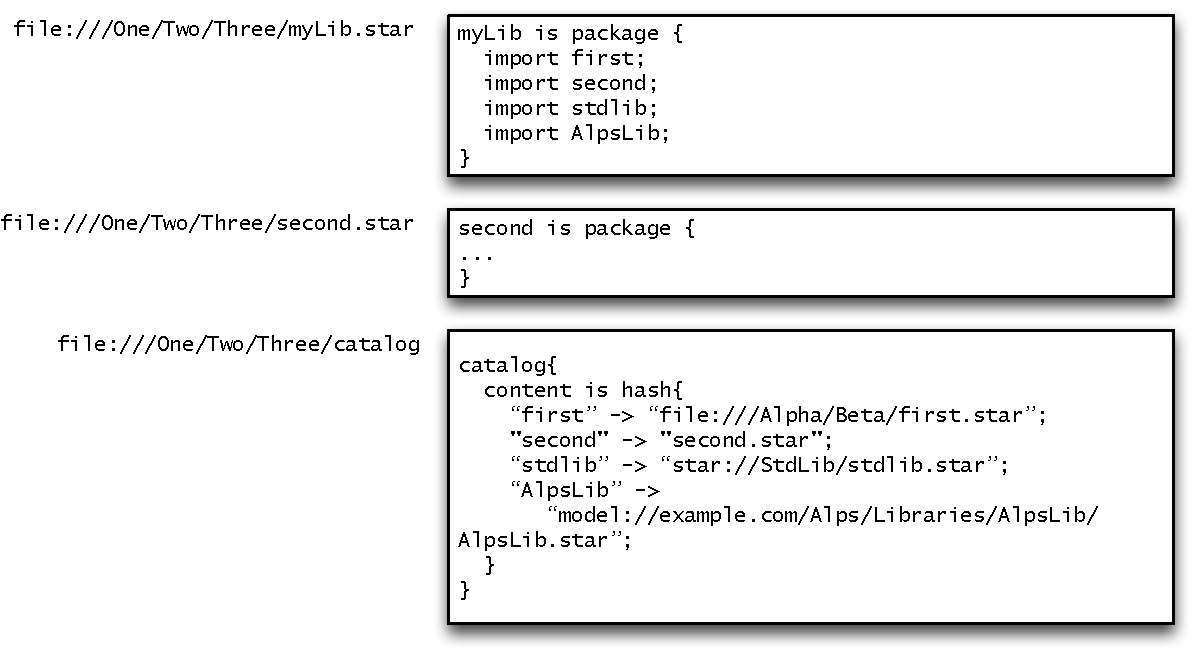
\includegraphics[width=\textwidth]{diagrams/library}
\caption{Library Structure}
\label{libraryFig}
\end{center}
\end{figure}

The library driver package typically has a standard form: it consists of a series of \ntRef{ImportStatement}s. The library is, in effect, defined by these \q{import}s.

The normal semantics of an \q{import} statement imply that the contents of all the \q{import}ed packages will be `re-exported' by the library driver package. The effect is that when the library driver package is imported, the entire contents of the library will be imported.

The second element of a library structure is the catalog. This typically contains the mapping from the names of packages to their URIs within the library `directory'.

Following the standard process of determining the catalog and URI of an \q{import}ed package, when the library driver \q{package} is imported, the library catalog will be accessed in order to interpret the contents of the library driver \q{package}.

\section{Resources and Catalogs}
\label{resources}

A package is an instance of a resource. A resource is any entity that can be identified. Examples of resources include package files (both source and compiled), and libraries. Resources need not be �static�: in principle, a service or a running application may also be viewed as a resource. However, in respect to the \Sr language, we are mostly concerned with \Sr package resources.

\subsection{Identifying Resources}
\index{Unified Resource Identifier}
The standard for identifying resources is the URI \cite{rfc2396}. \Sr uses URIs to locate source packages. Specifically, the \Sr language system \emph{must} support the URI schemes identified in Table~\vref{standardURISchemes}; however, it is free to support other schemes.

Program~\vref{uriProg} gives the \Sr definition of the standard \q{uri} type. This structure reflects the standard structure of a so-called hierarchic URI.  In addition to the `unpacked' \q{uri} structure, the \ntRef{TypeCoercion} expression:

\begin{lstlisting}
"..." as uri
\end{lstlisting}
represents a convenient way of writing URIs. The standard notation for URIs for supported schemes is supported by such expressions.

\begin{program}
\begin{lstlisting}
type uri is uri{
  scheme has type string;
  authority has type uriAuthority;
  path has type string;
  query has type string;
  fragment has type string
}

type uriAuthority is authority{
  user has type string;
  host has type string;
  port has type integer
} or noAuthority;
\end{lstlisting}
\caption{The Standard \q{uri} Type Description}\label{uriProg}
\end{program}

\begin{aside}
When a \q{uri} is used to denote an \q{import}ed package, the last part of the path must reflect the package name. I.e., if a package is called \q{pkg}, then the \q{uri} path must terminate in \q{.star}.
\end{aside}

\paragraph{Query Structure}
The \q{query} portion of a URI should take the form of a sequence of key=value pairs, separated by semi-colons. For example, a file URI with a VERSION attribute will look like:
\begin{lstlisting}
file:///foo/bar.star?VERSION=1.3;ACCESS=public
\end{lstlisting}

\subsubsection{Standard URI Schemes}
\label{standardSchemes}
The compiler recognizes a number of URI schemes as `standard': i.e., the compiler knows how to access the identified resources. In addition, the compiler also supports a technique for extending the set of known schemes with methods for locating the resources.
\begin{aside}
Technically, a URI contains no reliable indication of the physical location of the identified resource. However, for practical purposes it is often convenient to encode assumptions about physical location.
\end{aside}

The standard schemes supported by the compiler are listed in Table~\vref{standardURISchemes}.

\begin{table}[H]
\caption{Standard URI Schemes}\label{standardURISchemes}
\begin{center}
\begin{tabular}{|lll|}
\hline
Scheme&Type&Physical Location\\
\hline
\q{file:}&Local file&File path on system\\
\q{std:}&Built-in&Internal to compiler\\
\q{http:}&HTTP URL&Web page\\
\q{\$quoted\$:}&Quoted URI&Within URI's fragment\\
\q{star:}&Star source&File on local system\\
\hline
\end{tabular}
\end{center}
\end{table}

\begin{description}
\item[\q{file:}]A \q{file:} URI takes the form:
\begin{alltt}
file://\emph{Computer}/\emph{FilePath}
\end{alltt}
If the \emph{Computer} is omitted then the current machine that the compiler is executing on is assumed. If the \q{Computer} is not omitted, it may not be possible to access the remote computer.
\item[\q{std:}] A \q{std:} URI refers to resources that are properly part of the compiler itself. This are `hard-coded' in the sense that their location is established when the compiler is installed.
\item[\q{star:}] A \q{star:} URI refers to the default location that the compiler uses to find source files. This is often simply the working directory of the compiler; but may be configured with a command-line option.
\item[\q{http:}] A \q{http:} URI refers to a standard WEB URL. The compiler will attempt to access the resource by means of an HTTP request to the identified URL.
\item[\q{\$quoted\$:}] A \q{\$quoted\$} contains the source within the URI itself.

For example, the URI:
\begin{alltt}
$quoted$://hello#hello\%20is\%20package\%7b\%0a\%20\%20fun\%20hello
                                \%28\%29\%20is\%20\%22hello\%22\%3b\%0a\%7d
\end{alltt}
denotes the package:
\begin{lstlisting}
hello is package{
  fun hello() is "hello";
}
\end{lstlisting}
\begin{aside}
The standard notation for URIs requires that all the special characters used in a typical \Sr source must be encoded as \q{\%} hex pairs.

This URI is shown on two lines for convenience of display, but must actually be a contiguous sequence of characters.
\end{aside}
\begin{aside}
It is possible, if slightly redundant, to use quoted URIs to import a package:
\begin{lstlisting}
...
import "$quoted$://hello#hello%20is%20package
                 %7b%0a%20%20fun%20hello%28%29%20is%20%22
                 hello%22%3b%0a%7d";
...
\end{lstlisting}
However, a more important use of quoted URIs is to support dynamically compilation of \Sr in cases where the compiler is embedded.
\end{aside}
\end{description}

\subsubsection{Defining New Resource Schemes}
\label{newResoureScheme}
A new resource scheme may be introduced as a command line parameter using the \q{-DTRANSDUCER=} flag (see Section~\vref{compileFlags}).

The value of this flag is special form rule that takes the form:
\begin{alltt}
\emph{Ptn}==>\emph{Repl}
\end{alltt}
The syntax accepted by the pattern of the rule is the same as \ntRef{RegularExpression}; in particular, named groups are supported.

The purpose of this rule to map a new form of URI scheme into a predefined one.

In fact, the normal \q{star:} scheme can be expressed using a \q{TRANSDUCER} rule of the form:
\begin{alltt}
"star:(.*/)?([^/]+:V)==>file://\emph{tgtDir}/$V"
\end{alltt}
where \q{tgtDir} is the directory selected for finding source \Sr programs.

This particular rule locates the path component of the \q{star:} URI and translates it to a \q{file:}-based URI. It does not permit either a query or a fragment specifier; although these could be added they would have to be ignored.


\subsubsection{Resource Versions}
\label{uriVersion}
A resource URI may have a version indicator that identifies a particular version of the resource. The version indicator is a value associated with the \q{VERSION} keyword in the query portion of the URI.

For example, to specify version 2.1 of a resource, one might use the URI:
\begin{alltt}
file:///foo/bar.star?VERSION=2.1
\end{alltt}

The notation for version number is based on a release-version-update scheme.
\begin{figure}[htbp]
\begin{eqnarray*}
\ntDef{Version}&\arrow&\ntRef{Release}[\q{.}\ntRef{Version}[\q{.}\ntRef{Update}]]\\
\ntDef{Release}&\arrow&\ntRef{Digit}\sequence{}\ntRef{Digit}\\
\ntDef{Version}&\arrow&\ntRef{Digit}\sequence{}\ntRef{Digit}\\
\ntDef{Update}&\arrow&\ntRef{Digit}\sequence{}\ntRef{Digit}
\end{eqnarray*}
\caption{Version Numbering}
\label{versionNumberScheme}
\end{figure}
Version numbers are numeric, alphabetic version numbers are not permitted.

The requirement for any transducer that accesses a URI is either:
\begin{itemize}
\item if the URI references a specific version then that version of the resource should be accessed by the transducer;
\item if the URI does not reference a version, and if there are multiple versions of a resource, then the transducer must access the resource with the largest version number associated with it.
\end{itemize} 


\subsection{Packages and Paths}
\label{packagePath}
The URI used to identify a package must identify the package's name. Specifically, if the path component of a URI takes the form:
\begin{alltt}
Dir/Dir\sequence{/}Name.\emph{Ext}
\end{alltt}
then the name of the package -- as identified within the package source -- must be the same as the \q{Name} part of the package's URI.

This can be expressed more precisely as the substring of the URI's path gotten by removing both any leading folder names (separated by \q{/} characters) and any trailing extension (denoted as the remaining text following the last occurrence of a \q{.} character) must be the same as the name identified within the package source.

\subsection{Catalogs}
\label{catalog}
A catalog is a mapping from logical names to URIs. The \Sr language system uses this mapping to locate source files and compiled code when the corresponding resource is \q{import}ed by name. 

Catalogs offer an additional `level of indirection� between a name and the named entity. This indirection can be used, for example, to implement versioned access to resources. In addition, catalogs serve the role of �pulling together� the resources that a program or application needs into a coherent set.

Thus, when a package is imported by name, as in:
\begin{alltt}
world is package\{
  import hello;
  \ldots
\}
\end{alltt}
then the \Sr language system uses the catalog mapping to resolve the name \q{hello} to a \q{uri} in order to actually access the package. The \Sr type of \q{catalog} is shown in Program~\vref{catalogProg}.

\begin{program}
\begin{alltt}
type catalog is catalog\{
  content has type dictionary of (string,uri);
  version has type string;
  version default is nonString;
\}
\end{alltt}
\caption{The \q{catalog} Type}\label{catalogProg}
\end{program}

For example, the catalog definition:
\begin{alltt}
myCatalog is catalog\{
  content is dictionary of \{
    "hello" -> "file:///First/Second/hello.star";
    "stdlib" -> 
       "http://www.star-lang.org/extensions/StdLib/stdlib.star";
    "AlpsLib" -> 
       "model://example.com/Alps/Libraries/AlpsLib/AlpsLib.star";
    "star" -> "std:star.star"
  \}
\}
\end{alltt}
is a typical catalog denoting the programs available to a \Sr application. 

\subsubsection{Accessing Packages Using Catalogs}
\index{accessing packages with catalogs}
\index{catalog!accessing packages with}
The process of accessing a package involves:
\begin{enumerate}
\item If the package is identified by name, the URI of the package is looked up within the `current' catalog.
\begin{enumerate}
\item If the name is not present in the catalog, a fall-back catalog is searched if available.
\item If the name is not present, and there is no fall-back, exit with an error.
\end{enumerate}
\item The located URI is resolved against the URI of the current catalog. This allows catalogs themselves to contain relative URIs where possible.  This is the so-called target URI.

\item The target URI is dereferenced -- using a transducer -- and accessed. If the resource does not exist, or is not valid, exit with an error.
\item The catalog uri:
\begin{alltt}
"../catalog"
\end{alltt}
is resolved against the URI of the package containing the reference.
\begin{enumerate}
\item If a catalog exists in this location then that catalog is used to resolve references within the target resource.
\item If there is no catalog, then a catalog \emph{may} be synthesized by `exploring' the space around the target URI.
\end{enumerate}
\end{enumerate}

\subsubsection{Multiple Versions of a Package}
A code repository may contain multiple versions of a package. A programmer may specify a specific version to import by specifying the version in the package's URI: either directly in the \ntRef{ImportStatement} or in the catalog.

If no version is specified, then importing a package will always reference the package in the repository with the largest version number.

When compiling a package, the version of the package may be specified as a command-line option to the compiler or by defining a non-trivial value for the \q{version} attribute in the catalog structure.

However specified, the versions that a package is compiled against are fixed during the compilation of the package. I.e., when a package is compiled, it is compiled against specific versions of imported packages. When the package is later executed, the specific versions that were accessed at compile time are also used at run-time.
